
\begin{theorem} \textbf{Teorema de Green.} \label{green}  Sean $U\subseteq \Rn{2}$ abierto  y   $D \subsetneq  U$ un conjunto  simplemente conexo (\autoref{def:conjuntoconexo_simp}) cuyo borde, $\partial D$, es una curva simple y cerrada.  Si  $\mathbf{F}:U\to\Rn{2}$ es de clase $\mathcal{C}^1$, entonces
    \[
        \oint_{\partial D^{+}} \mathbf{F}\cdot d\mathbf{s} = \iint_D \grad\times\mathbf{F}\cdot d\mathbf{A}.
    \]
\end{theorem}

\begin{obs} Sea $\mathbf{F}:U\subset \Rn{2}\to\Rn{2}$ bajo las condiciones de (\ref{green})  con $\mathbf{F}=(P,Q)$,  el teorema de Green  puede ser escrito de siguiente manera alternativa:
\[
    \oint_{\partial D^+}P\:dx+Q\:dy=\iint_D\left(\dif{Q}{x}-\dif{P}{y}\right)dA,
\]
basta con ver la notaci\'on dada en (\ref{not_int}) y recordar que 
\[
    \nabla\times\mathbf{F} = \dif{Q}{x}-\dif{P}{y}.
\]
\end{obs}

\begin{tarea}
 Para  la curva simple, cerrada y orientada $C$ formada por los segmentos  de $(0, 0)$ a $(1, 1),$ de (1,1) a $(0, 1)$ y de $(0, 1)$ vuelta al $(0, 0)$, calcular  $$\int_{C} xy \; dx + \sqrt{y^{2}+1} \; dy.$$
\end{tarea}


\begin{tarea}
 Sea    $D=\{  (x,y) \in \mathbb{R}^{2} \: : \: 1 \leq x ^{2}+ y^{2}  \leq  4,  x\geq 0 \}$ , calcular   $$\int_{(\partial D)^{-}} x^{2}y \; dx - xy^{2} \; dy.$$
\end{tarea}


\begin{propertie}   Sean $U\subseteq \Rn{2}$ abierto  y   $D \subsetneq  U$ un conjunto  simplemente conexo  cuyo borde, $\partial D$, es una curva simple y cerrada.  Si  $\mathbf{F}:U\to\Rn{2}$ tal que $ \grad\times\mathbf{F} =1 $ entonces
    \[
        \oint_{\partial D^{+}} \mathbf{F}\cdot d\mathbf{s} =  A(D).
    \]
\end{propertie}

\begin{tarea}
Hallar el \'area de la regi\'on encerrada por la curva cerrada con parametrizaci\'on   $\sigma(t) = (\sin t \cos t, \sin t)$ con $0\leq t \leq \pi$.     


 

\begin{figure}[H]
\begin{center}
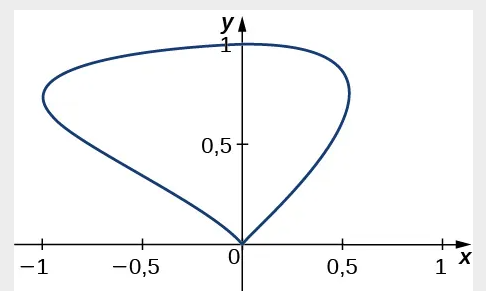
\includegraphics[scale=0.6]{figs/green.png}
\end{center}
\end{figure}
\end{tarea}

\newpage

\begin{obs}
    \textbf{Extensi\'on de Green.} El teorema de Green es aplicable a regiones a\'un m\'as generales que regiones simplemente conexas.  Dicho teorema puede ser adaptado a cualquier regi\'on en $\Rn{2}$ cuya frontera  se pueda descomponer en un n\'umero finito de curvas cerradas y simples.  La idea es ``recorrer" dicha frontera pasando por todas las curvas que la confroman. 

Veamos, a modo ilustrativo,  el siguiente ejemplo. Sea $D \subset \mathbb{R}^{2}$   el siguiente conjunto (pintado de violeta),  claramente $D$  no simplemente conexo. 
    
    \begin{center}
    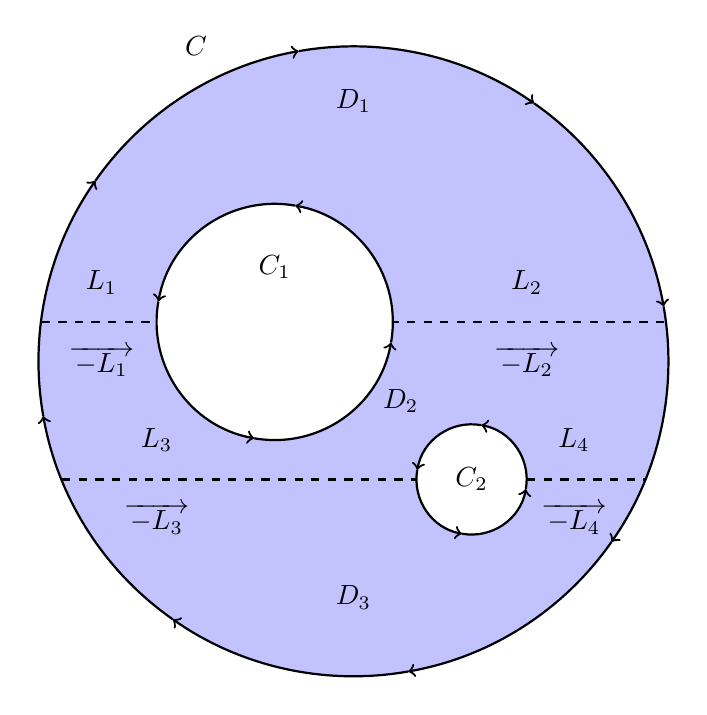
\begin{tikzpicture}
        % Define the exterior boundary with clockwise arrows
        \fill[blue!60!white!40] (0,0) circle (4);
        \foreach \angle in {315, 270, 225, 180, 135, 90, 45, 0} {
            \draw[thick, ->] ({4*cos(\angle+10)}, {4*sin(\angle+10)}) 
                arc[start angle=\angle+10, end angle=\angle-45+10, radius=4];
        }
        
        \draw[thick, dashed] (-3.96, 0.5) -- (3.96, 0.5);
        \draw[thick, dashed] (-3.7, -1.5) -- (3.7, -1.5);
        
        % Inner circle 1 with counterclockwise arrows
        \fill[white] (-1,0.5) circle (1.5);
        \foreach \angle in {0, 90, 180, 270} {
            \draw[thick, ->] ({-1+1.5*cos(\angle+80)}, {0.5+1.5*sin(\angle+80)}) 
            arc[start angle=\angle+80, end angle=\angle+170, radius=1.5];
            }
            
            % Inner circle 2 with counterclockwise arrows
        \fill[white] (1.5,-1.5) circle (0.7);
        \foreach \angle in {0, 90, 180, 270} {
            \draw[thick, ->] ({1.5+0.7*cos(\angle+80)}, {-1.5+0.7*sin(\angle+80)}) 
                arc[start angle=\angle+80, end angle=\angle+170, radius=0.7];
                }

        % Labels for regions
        \node at (0,3.3) {$D_1$};
        \node at (0.6,-0.5) {$D_2$};
        \node at (0,-3) {$D_3$};
        \node at (-2, 4) {$C$};
        \node at (-1,1.2) {$C_1$};
        \node at (1.5,-1.5) {$C_2$};
        \node at (-3.2, 1) {$\underleftarrow{\;\;L_1\;\;}$};
        \node at (-3.2, 0) {$\overrightarrow{\:-L_1\:}$};
        \node at (2.2, 1) {$\underleftarrow{\;\;L_2\;\;}$};
        \node at (2.2, 0) {$\overrightarrow{\:-L_2\:}$};
        \node at (-2.5, -1) {$\underleftarrow{\;\;L_3\;\;}$};
        \node at (-2.5, -2) {$\overrightarrow{\:-L_3\:}$};
        \node at (2.8, -1) {$\underleftarrow{\;\;L_4\;\;}$};
        \node at (2.8, -2) {$\overrightarrow{\:-L_4\:}$};
    \end{tikzpicture}
    \end{center}

El conjunto $D$ puede ser escrito como la uni\'on de tres conjuntos  disjuntos entre si (salvo tal vez en sus bordes) simplemente conexos,  $D_1$, $D_2$ y $D_3$, es decir,  $$D =D_1\cup D_2\cup D_3.$$  El borde de $D$ es la uni\'on de tres curvas cerradas simples,   $C$, $C_1$ y $C_2$, es decir,  $$\partial D=C\cup C_1\cup C_2.$$
Orientemos a la curva  $C$ en sentido horario y a las curvas  $C_1$ y $C_2$  en sentido  antihorario.  

Por lo tanto, si $\mathbf{F}$ es un campo vectorial definido en $D$, aplicando el teorema de Green.
    \begin{align*}
        \oint_{\partial D} \mathbf{F}\cdot d\mathbf{s}=&\oint_{C^{-}}\mathbf{F}\cdot d\mathbf{s}+\oint_{C_1^{+}}\mathbf{F}\cdot d\mathbf{s}+\oint_{C_2^{+}}\mathbf{F}\cdot d\mathbf{s}\\[.2cm]
        =&\oint_{\partial D_1^{-}}\mathbf{F}\cdot d\mathbf{s}+\oint_{\partial D_2^{-}}\mathbf{F}\cdot d\mathbf{s}+\oint_{\partial D_3^{-}}\mathbf{F}\cdot d\mathbf{s}\\[.2cm]
        =&-\iint_{ D_1}\grad\times\mathbf{F}\cdot d\mathbf{A}-\iint_{ D_2}\grad\times\mathbf{F}\cdot d\mathbf{A}-\iint_{ D_3}\grad\times\mathbf{F}\cdot d\mathbf{A}\\[.2cm]
        =&-\iint_D \grad\times\mathbf{F}\cdot d\mathbf{A}
    \end{align*}
\end{obs}

Se deja al lector los detalles del procedimiento anterior. 

\begin{tarea}
Sea $F(x,y) = (\dfrac{y}{x^{2}+y^{2}},\dfrac{-x}{x^{2}+y^{2}})$ y sea $C$ una curva en el plano, cerrada, simple y orientada en sentido antihorario. Calcular todos  los posibles valores de $\int_{C} F ds.$
\end{tarea}


\begin{theorem}
\textbf{Teorema de la divergencia en el plano.} Sea $D\subset\Rn{2}$ una regi\'on donde valga el teorema de Green y sea $\partial D$ su frontera. Denotaremos por $\mathbf{n}$ el versor unitario normal exterior a $\partial D$.  Si $\boldsymbol{\sigma}:[a,b]\to\Rn{2},\;\boldsymbol{\sigma}(t)=(x(t),y(t))$ es una parametrizaci\'on que recorre a $\partial D$ de manera positiva,  entonces  $\mathbf{n}$ est\'a dado por 
\[
    \mathbf{n}=\frac{(y'(t),-x'(t))}{\sqrt{[x'(t)]^2+[y'(t)]^2}}.
\]
Si $\mathbf{F}:  D\to \Rn{2}$ es un campo vectorial continuo y de clase $\mathcal{C}^1(\interior{D})$,  entonces
\[
    \int_{\partial D}\mathbf{F}\cdot\mathbf{n}\:ds=\iint_D\grad\cdot\mathbf{F}\:dA.
\]
\end{theorem}

\begin{theorem}
\textbf{Teorema de Stokes.}  Sean $\boldsymbol{\Sigma}:D\subset\Rn{2} \to S\subset\Rn{3}$    una parametrizaci\'on regular y  de clase  $\mathcal{C}^1(\interior{D})$ de una superficie $S$ y $A \subseteq \Rn{3}$ un conjunto abierto.    Si $\mathbf{F}:  A\subseteq \Rn{3}\to \Rn{3}$ es un campo vectorial continuo, de clase  $\mathcal{C}^1(A)$ tal que  $S \subsetneq A$, entonces
\[
    \oint_{\partial S}\mathbf{F}\cdot d\mathbf{s}=\iint_S\grad\times\mathbf{F}\cdot d\mathbf{S}, 
\]  donde las orientaciones tanto de  $S$ como de $\partial S$ son las inducidas por $\boldsymbol{\Sigma}$ sobre ellas, ver  (\ref{sigma_induce_1}) y  (\ref{sigma_induce}).
\end{theorem}

\begin{tarea} Sean  $S=\{  (x,y,z) \in \mathbb{R}^{3} \: : \:  x ^{2}+ y^{2} = z,  x ^{2}+ y^{2}  \leq 4 \}$  y $F(x,y,z) = (x ^{2}z^{2}, y^{2}z^{2}, xyz)$, calcular, indicando la orientaci\'on elegida   $$\iint_S\grad\times\mathbf{F}\cdot d\mathbf{S}$$
\end{tarea}

\begin{tarea} Sea  $C=\{  (x,y,z) \in \mathbb{R}^{3} \: : \:  z=4, \: x ^{2}+ y^{2}   = 4 \}$  una curva cerrada y simple y sea  $F(x,y,z) = (x ^{3}z^{3}+y, y^{\frac{1}{3}}z^{2}, xyz)$,  calcular,  indicando la orientaci\'on elegida,      $$\int_{C}\mathbf{F}\cdot d\mathbf{S}$$
\end{tarea}



\begin{theorem}
\textbf{Teorema de la divergencia o de Gauss.}  Sean $S\subset\Rn{3}$ una superficie que encierra un volumen $\Omega$, \textit{i.e.} $S=\partial \Omega$, orientada de manera exterior y $A \subseteq \Rn{3}$ un conjunto abierto .  Si $\mathbf{F}:A \subseteq \Rn{3} \to\Rn{3}$ es  un campo vectorial continuo y de clase $\mathcal{C}^1(A)$ tal que $\Omega \subsetneq A$, entonces
\[
    \oiint_{\partial \Omega}\mathbf{F}\cdot d\mathbf{S}=\iiint_{\Omega}\grad\cdot\mathbf{F}\:dV.
\]
\end{theorem}


\begin{tarea}
 Probar que el flujo de $\mathbf{F} = (ax, by, cz)$ con $a,b,c \in \mathbf{R}^+$ a través del cubo: $V : [-1,1] \times [-1,1] \times [-1,1]$ orientado con normales salientes es $(a+b+c) \mathrm{volumen}(V)$.
\end{tarea} 


\begin{tarea}
 Sea la superficie   $S=\{  (x,y,z) \in \mathbb{R}^{3} \: : \: x ^{2}+ y^{2} = z^{2}, 1 \leq z \leq 2 \}$   y   sea el campo $F(x,y,z)=(x+y^{2}z^{2}, y+z^{2}x^{2}, z).$  Hallar el flujo  de $F$ a trav\'es de $S$ indicando la orientaci\'on elegida.
\end{tarea}  



\begin{tarea}
Sea  $S=\{  (x,y,z) \in \mathbb{R}^{3} \: : \: x ^{2}+ y^{2} +1= z,  \:  1\leq z \leq h\}$  y sea  el campo $F(x,y,z)=(z+y^{3},  y+ \cos (z^{2}x^{2}),  -z).$    Hallar $h \in \mathbb{R}$ tal que: $$\int_{S} F . dS = 2\pi. $$  Indicar la orientaci\'on con la cual resuelve el ejercicio.
\end{tarea}